\documentclass{standalone}
\usepackage{tikz}
\usetikzlibrary{shapes.geometric, arrows.meta}

\tikzstyle{factor} = [rectangle, draw=black, fill=white, text width=4em, text centered, rounded corners, minimum height=1em]
\tikzstyle{decision} = [diamond, draw=black, fill=white, text width=4em, text badly centered, inner sep=0pt]
\tikzstyle{arrow} = [thick,->,>=stealth]

\begin{document}

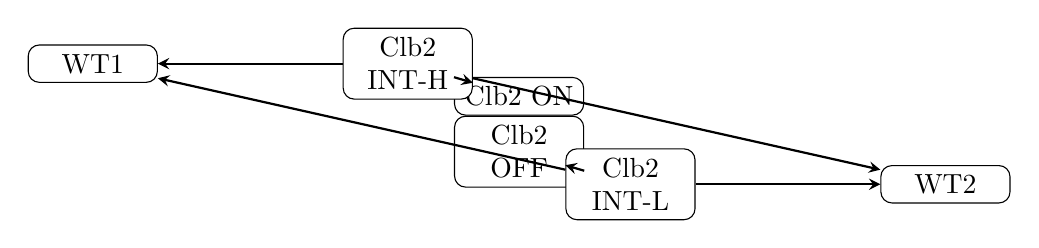
\begin{tikzpicture}[node distance=2cm]

    % Nodes
    \node (Clb2ON) [factor, above] {Clb2 ON};
    \node (Clb2OFF) [factor, below] {Clb2 OFF};
    \node (Clb2INTH) [factor, above left of=Clb2ON, yshift=-1cm] {Clb2 INT-H};
    \node (Clb2INTL) [factor, below right of=Clb2OFF, yshift=1cm] {Clb2 INT-L};
    \node (WT1) [factor, left of=Clb2INTH, xshift=-2cm] {WT1};
    \node (WT2) [factor, right of=Clb2INTL, xshift=2cm] {WT2};

    % Edges
    \draw [arrow] (Clb2ON) -- (Clb2INTH);
    \draw [arrow] (Clb2OFF) -- (Clb2INTL);
    \draw [arrow] (Clb2INTH) -- (WT1);
    \draw [arrow] (Clb2INTH) -- (WT2);
    \draw [arrow] (Clb2INTL) -- (WT1);
    \draw [arrow] (Clb2INTL) -- (WT2);

\end{tikzpicture}

\end{document}